%\documentclass[a4paper,twoside,10pt]{article}
\interfootnotelinepenalty=10000
\usepackage[USenglish]{babel} %francais, polish, spanish, ...
\usepackage[T1]{fontenc}
%\usepackage[ansinew]{inputenc}
\usepackage{color}
\usepackage{mathtools}
%\usepackage{hyperref}
\usepackage{subfig}
\usepackage{multirow, booktabs}
\usepackage{hyperref}


\usepackage{lmodern} %Type1-font for non-english texts and characters
\usepackage{algorithm}
\usepackage[noend]{algpseudocode}
\usepackage{mnsymbol}

%% Packages for Graphics & Figures %%%%%%%%%%%%%%%%%%%%%%%%%%
\usepackage{graphicx} %%For loading graphic files
\usepackage{amsmath}
\usepackage{amsthm} 
\usepackage{thmtools}
\usepackage{amsfonts}
\usepackage[all,cmtip]{xy}
\usepackage{tikz}

\usepackage{TechFront}
%\declaretheorem{Lemma}
%\declaretheorem{prop}

\newcommand{\lre}{\color{red}{\{}}

%\DeclareMathOperator{\sign}{sgn}
%\DeclareMathOperator{\coef}{coef}
%\DeclareMathOperator{\var}{var}
%\DeclareMathOperator{\eqs}{eqs}
%\DeclareMathOperator{\feas}{feas}
%\DeclareMathOperator{\UB}{UB}
%\DeclareMathOperator{\lb}{lb}
%\DeclareMathOperator{\FMcomb}{FM-comb}
%\DeclareMathOperator{\Gcomb}{Gauss-comb}
%\DeclareMathOperator{\proj}{proj}
%\DeclareMathOperator{\Pos}{Pos}
%\DeclareMathOperator{\Neg}{Neg}
%\DeclareMathOperator{\rhs}{rhs}
\newcommand{\sign}{\mathit{sgn}}
\newcommand{\coef}{\mathit{co}}
\newcommand{\var}{\mathit{var}}
\newcommand{\VAR}{\mathit{VAR}}
\newcommand{\eqs}{\mathit{eqs}}
\newcommand{\feas}{\mathit{feas}}
\newcommand{\UB}{\mathit{UB}}
\newcommand{\UBc}{\mathit{UBineq}}
\newcommand{\lb}{\mathit{lb}}
\newcommand{\lbc}{\mathit{lbineq}}
\newcommand{\FMcomb}{\mathit{FM}}
\newcommand{\Gcomb}{\mathit{GA}}
\newcommand{\proj}{\mathit{proj}}
\newcommand{\Pos}{\mathit{Pos}}
\newcommand{\Neg}{\mathit{Neg}}
\newcommand{\rhs}{\mathit{rhs}}
\newcommand{\bounds}{\mathit{bounds}}
\newcommand{\ie}{\mathcal{IE}}
\newcommand{\xx}{\mathcal{X}}
\newcommand{\vea}{\mathbf{co}}
\newcommand{\ttt}{\texttt{t}}
\newcommand{\trt}[1]{\texttt{#1}}
\newcommand{\mi}{\mathit}

\newcommand{\false}{\texttt{false}}
\newcommand{\true}{\texttt{true}}
\newcommand{\nul}{\texttt{null}}
\newcommand{\ve}{\mathbf}
%\newcommand\lhs[1]{\text{lhs}(#1)}
%\newcommand\rhs[1]{\text{rhs}(#1)}
%\newcommand\coef[1]{\text{coef}(#1)}
%\newcommand\LB[1]{\text{LB}_{#1}}
%\newcommand\UB[1]{\text{UB}_{#1}}
\newcommand{\lig}[4]{\ve{#1}\cdot\ve{#2}#3#4}
\newcommand\red[1]{\textcolor{red}{#1}}
\newcommand\blue[1]{\textcolor{blue}{#1}}
\newcommand{\set}[2]{\{\;{#1}\;|\;{#2}\;\}}
\newcommand{\odef}{\overset{\text{def.}}=}
\newcommand{\mc}{\mathcal}
\algdef{SE}[DOWHILE]{Do}{doWhile}{\algorithmicdo}[1]{\algorithmicwhile\ #1}%
\newcommand{\argmin}{\operatornamewithlimits{argmin}}
\newcommand{\StateInd}{\State\hspace{\algorithmicindent}}
\newcommand{\pr}{\mathit{PR}}
\newcommand{\prs}{\mathit{PRS}}
\newcommand{\ens}{\Leftrightarrow}

%\algdef{SE}[DOPAR]{DoPar}{doParWhile}{\algorithmicdo\textbf{ in parallel for\ }}[1]{\algorithmicwhile\ #1}%
\algdef{SE}[DOPAR]{DoPar}{doParUntil}{\algorithmicdo\textbf{ in parallel for\ }}[1]{\algorithmicuntil\ #1}%

\algdef{SE}[SUBALG]{Indent}{EndIndent}{}{\algorithmicend\ }%
\algtext*{Indent}
\algtext*{EndIndent}

\newtheorem{prop}{Proposition}
\newtheorem{lemma}{Lemma}
\newtheorem{cor}{Corollary}

\newcounter{para}
%\newcommand\mypara[1]{\par\refstepcounter{para}\textbf{\thep‌​ara\space#1\space}}
\newcommand\mypara[1]{\newline\par\refstepcounter{para}\textbf{\thepara}\space \textbf{#1} \space}
%\newcommand\mypara{\par\refstepcounter{para}\thepara\space}
%\usepackage[thmmarks,...]{ntheorem}
\newcommand{\Sec}{F}
\newcommand{\Ca}{\mi{Cap}}
\newcommand{\Vol}{\mi{V}}
\newcommand{\Weight}{\mi{W}}
\newcommand{\weight}{\mi{w}}
\newcommand{\BonjeanStations}{\mi{BS}}
\newcommand{\bonjean}{bf}
\newcommand{\Bonj}{B}
\newcommand{\shear}{\mi{sf}}
\newcommand{\Prop}{P}

\theoremstyle{definition}
%\newtheorem{example}{Example}[section]
\newtheorem*{theorem}{Theorem}

\theoremstyle{definition}
\newtheorem{examplex}{Example}[section]
\newenvironment{example}
  {\pushQED{\qed}\renewcommand{\qedsymbol}{$\triangle$}\examplex}
  {\popQED\endexamplex}
	
%\newtheoremstyle{named}{}{}{\itshape}{}{\bfseries}{.}{.5em}{\thmnote{#3}}
%\theoremstyle{named}
%\newtheorem*{namedtheorem}{Theorem}

%\begin{document}

\section{Results}\label{sec:results}
%\subsection{What has been done}
From data for a specific vessel, we have constructed a number of different models, where the weight and hydrostatics are taken into account to various degrees. The first model does not consider the weight of the containers at all (i.e. the described constraints limiting the total displacement as well as all hydrostatic constraints have been removed), the second model does not model any hydrostatic constraints, and the subsequent models consider the hydrostatic constraints at 2, 4, 6 and 8 measure points, respectively.

Each model has been projected, such that only the variables denoting the number of each type of containers is left, that is, all variables but $\set{x_\tau}{\tau\in T}$ are eliminated. 
Projections have been done in two different ways, decomposed and flat. For the decomposed projections, a tree structure has been used as described in Section~\ref{sec:decomp}, while the flat projection does not use any decomposition at all. %\red{The particular used decompositions can be found in the appendix}. 
Our algorithms have been implemented in Java, and the projections were done on a computer with an {Intel\textsuperscript{\textregistered} Xeon\textsuperscript{\textregistered} E5-1660 V4 processor with a frequency of 3.20-3.80 GHz, 32GB RAM, and with 8 cores and 16 threads.}

The original and the projected models have been optimized for revenue, and objective value as well as time taken has been compared. The latter is measured in both iterations and \emph{ticks} as it appears when solved with CPLEX Interactive Optimizer version 12.5.0.0. Ticks is a deterministic time measure that according to the software provider ``yields the same level of performance for repeated solving of the same model with the same parameter settings, on the same computing platform''\footnote{\url{https://www.ibm.com/support/knowledgecenter/SSSA5P_12.5.0/ilog.odms.studio.help/CPLEX/ReleaseNotes/topics/releasenotes125/newDetTime.html, March 22, 2018}}. 
The revenue is dependent on the container type, so that the container types that (in the industry) are found more limiting also yields a higher revenue, see further below. 

\subsection{Size reduction}
Table~\ref{tab:projections} summarizes the size of the original (unprojected) VSMs and the projected models that are the result of the projection using decomposition. These sizes are given in terms of the number of inequalities (ineqs), variables (vars), non-zero entries (nzs.) and density (dens.). The size of the original models are given both as they appear as input to our algorithm, but also after a {competitive} preprocessing, namely after it has been preprocessed by CPLEX. For comparison, the table includes the simple capacity model for the particular vessel we have used. This model is the one currently used in the industry, and it only includes upper bounds on the total number of containers, the total number of reefer containers, and the total weight.  

\begin{table}[htbp]
\centering
\begin{tabular}{l|r@{ / }r@{ / }r@{ / }r|r@{ / }r@{ / }l@{ / }r|r@{ / }r@{ / }r@{ / }r}%|rr}
\toprule
$\multirow{2}{*}{Model}$&\multicolumn{4}{c|}{Original size}&\multicolumn{4}{c|}{Original, presolved}& \multicolumn{4}{c}{Projected size}\\%&\multicolumn{2}{c}{Time}\\
&ineqs (eqs)&vars&nzs.& dens.&rows&cols&nzs.&dens.&ineqs&vars&nzs.&dens.\\%&decomp.&flat\\
\midrule
{No weights} &774 (12)&1142&6662&8.61&	554&657&2784&5.03&				20&12&\phantom{1}155&7.75\\ %27.7, 
{No hydro.} &806 (43)&1173&7854&9.74&	555&657&3441&6.20&		18&12&\phantom{1}144&8.00 \\ % 30.83
{2 parts} &810 (43)&1173&7860&9.70&	556&661&3447&6.20&					96&12&1113&11.59\\ % 5.79
{4 parts} &824 (49)&1179&7886&9.57&	564&671&3471&6.15&	64&12&\phantom{1}731&11.42\\% 8.81
{6 parts} &838 (55)&1185&7916&9.44&	570&679&3496&6.13&	80&12&\phantom{1}888&11.10\\% 7.125
{8 parts} &852 (61) &1191 &7950&9.33	&	576&685&3522&6.11&	52 &12&\phantom{1}582&11.19\\% 11.08
\bottomrule
\multicolumn{10}{c}{}\\
\cmidrule{1-9}
Simple model & 3&12 &\phantom{12}36&12.00&3&9&\phantom{12}24&\multicolumn{1}{l}{8.00}\\
\cmidrule{1-9}
\end{tabular}
\caption{The size of the systems (VSMs), before and after projection, given in terms of the number of inequalities (ineqs), variables (vars), non-zero entries (nzs.), and density (dens.) The size of the simple capacity model is included for comparison. }
\label{tab:projections}
\end{table}
The results show that the projected models have much fewer inequalities and variables, namely app. 6 - 30 times fewer inequalities and 54-57 times fewer variables than even the presolved systems. The projected systems also have fewer non-zero entries (between 3 and 24 times fewer), though, the projected models are more dense (app. 1.3 to 1.9 more dense than the presolved systems).

The results reveal no apparent relationship between the size of the original model and the size of the projection, which probably have to do with both the actual position of the hydrostatic measure points and the undeterministic behaviour of the removal of almost redundant inequalities. 

\subsection{Decomposition}
Table~\ref{tab:time} shows the time taken for the algorithm to do the projection, both decomposed and flat. For most models, the flat projection timed out (TO) after 65 hours, in which case the variables left to be projected is given.
Figure~\ref{fig:8parts} shows the progression of the number of inequalities and variables, respectively, as a function of time when the algorithm runs on the decomposed 8 part-model. These numbers are the sum of all the inequalities and variables, respectively, in all the projected or unprojected subsystems in the decomposition at a given time. Likewise, Figure~\ref{fig:compare} shows the progression for the flat projection of the same model; this figure includes the number of inequalities for the decomposed projection for comparison. Each graph shows the number of inequalities and variables after the preprocessing step, each Gauss-elimination, and each FM-elimination followed by some preprocessing, parallel redundancy removal and sequential removal of almost redundant inequalities.    
\begin{table}[htbp]
\centering
\begin{tabular}{l|r@{\hspace{-3em}}rc|rc}
\toprule
$\multirow{2}{*}{Model}$&\multicolumn{5}{c}{Time}\\
&\multicolumn{2}{r}{decomp.}& vars left to project&flat&vars left to project\\
\midrule
{No weights}& &24.5m&-&2.5m&-\\% (and it's smaller)\\ 24m 36s 2m 30s
{No hydro.}& &14.5m&-&1.8m&-\\% (!) (and it's smaller)\\14m29s%4h 35m 59s&1m 48s
{2 parts} &7h&18m &-&(TO) 32h& 551\\%7h 17m 59s, 563
{4 parts} &8h&4m &-&(TO) 61h & 557\\%8h 4m 0s, 569
{6 parts} &3h&7m &-&(TO) 18h & 577\\%3h 7m 0s, 589
{8 parts} &3h&19m &-&(TO) 65h& 566\\ %3h 18m 37s, 578
\bottomrule
\end{tabular}
\caption{Time taken to do the projections, using decomposition or not (flat), respectively. The time limit is set to 65 hours.}
\label{tab:time}
\end{table}

From the results in Table~\ref{tab:time}, it is clear that the decomposition has a huge impact on the success of the projection algorithm when the system includes
%has a none-negligible number of ``interacting'' global constraints as the models with 
hydrostatic constraints.
The table also shows, that the two smallest systems that does not take hydrostatic constraints into consideration are solved faster using a flat projection. This behaviour is not surprising, since the hydrostatic constraints are dense, global constraints that links the weight of all sections to the left or right of a measure point, and the coefficients in the constraints are non-trivial. Thus, when these are included, decomposition is extremely useful while not necessary for the simpler systems.
 
\begin{figure}[htbp]
	\centering
		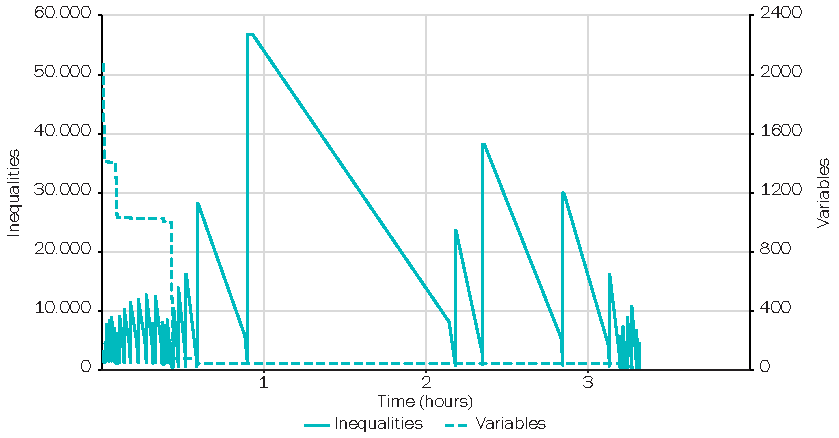
\includegraphics{figures/decompIneqGrowth.pdf}
	\caption{The inequalities growth and variable decrease for the 8 part-model with decomposition.}
	\label{fig:8parts}
\end{figure}

\begin{figure}[htbp]
	\centering
		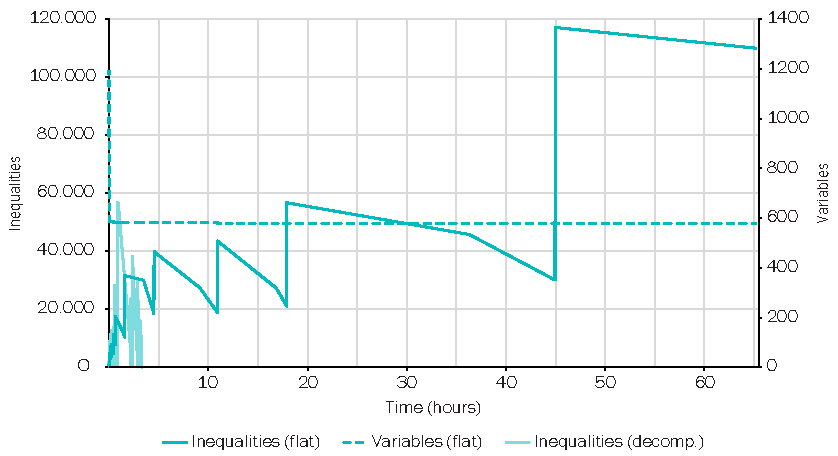
\includegraphics{figures/ineqGrowth.pdf}
	\caption{The inequalities growth for the 8 part-model with and without decomposition.}
	\label{fig:compare}
\end{figure}

When considering each subsystem in a decomposition as a system in itself, in general, the number of inequalities after each call to \Call{FME-SingleVar}{} in Algorithm~\ref{alg:FMEF} grows to begin with, as does the number of inequalities before this call. This continues until there are a few variables left, where both these numbers decrease. Notice, that the graph in Figure~\ref{fig:8parts} shows the total run of the projection algorithm, causing this pattern to be repeated. Hence it may be hard to see this in the figure.

For the decomposed algorithm, though the number of inequalities grow after each FME-step, most of them are redundant or almost redundant. The same does not hold for the flat projection for the cases where hydrostatics are taken into consideration, at least not for the FME-steps that are completed within the time limit. Instead, many of the produced inequalities are non-redundant which increases the likelyhood that even more inequalities will be produced in the next elimination, but also that the redundancy removal will take longer time - not only are there more inequalities to check, each check will also take longer. 
{Though this is just speculations, since the flat projections were not finished due to time and memory constraints, it appears that the flat projection of the total system on a ``global'' scale behaves as an ``enlarged'' version of described pattern for the subsystems.}

{This behavior can be explained by the occurrence of several ``interacting'' global constraints: the algorithm projects a few variables from one subsystem (resulting in a little denser global constraints) before moving on to the next subsystem from where it removes another few variables etc., all the while it postpones dealing with the variables in the global inequalities which get more and more dense.}

It should be mentioned that it is possible, that other orderings of the variables (caused by other heuristics then the used greedy heuristic) in these cases could potentially lead to manageable flat projections, but testing this is outside the scope of this paper.  
We also note that the runtime, even for the decomposed projections, are not exactly small, and the main part of the execution time is spend doing redundancy removal. However, as mentioned in the introduction, these calculations are off-line that should be done once, after which they can be used as submodels in other optimization models.  

\subsection{Revenue optimization}
The original and the projected models have been optimized for revenue using CPLEX. 
Each transported container yields a revenue which is based on its type, i.e. on the size, weight and reefer-property of the container. More specifically, for our tests, reefer containers yields the double revenue as a similar non-reefer container, 40' containers have a revenue which is 1.5 times higher as a similar 20' container, while containers are more expensive the heavier it is. A 20', non-reefer container, with a weight, respectively of 6, 21, and 27 ton, is assigned the following revenue in USD: 100, 600 and 700, respectively.   

Table~\ref{tab:usingProjections} shows the number of iterations, the deterministic time and the objective value found by CPLEX when optimizing revenue for the original and projected models. It likewise shows how many times faster, the projections are w.r.t. iteration and ticks, as well as the difference in objective value in percentage. For comparison, the number of iterations, deterministic time and objective value is shown too for the simple model, which was mentioned previously. %\red{[I should compare with the naive model as well, but I don't see how I should do that]}

\begin{table}[htbp]
\centering
\begin{tabular}{l|rrr|rrr|rrr}
\toprule
Model&\multicolumn{3}{c|}{Projected}&\multicolumn{3}{c|}{Original}&\multicolumn{3}{c}{Difference}\\
&Iter.&Ticks&Objective&Iter.&Ticks&Objective&Iter. (times)&Ticks(times)&Obj.(\%)\\ %(Phase 1 iterations)
\midrule
No weights&	11 & 0.05 & $8.63\cdot 10^6$ &	363 & 2.64&$8.08\cdot 10^6$
&33.0&52.8&6.8\\
%No weights&	11(0) & 0.05 & $8.6318\cdot 10^6$ &	363(92) & 2.64&$8.0802\cdot 10^6$ &96.97&98.12&6.83\\
\midrule
{No hydro.}& 9 & 0.04 &$7.87\cdot 10^6$&	188 & 5.48&$6.22 \cdot 10^6$
&20.9&137&26.5\\
%{No hydro.}& 7(0) & 0.03 &$6.2217\cdot 10^6$&	188(1) & 5.48&$6.2215 \cdot 10^6$ &96.28&99.45&0.0032\\
\midrule
{2 parts}& 14 & 0.29 & $6.09\cdot 10^6$ &	251 & 5.88&$6.07\cdot 10^6$
&17.9&20.3&0.196\\
%{2 parts}& 14(0) & 0.29 & $6.0862\cdot 10^6$ &	251(2) & 5.88&$6.0743\cdot 10^6$ &94.42&95.07&0.1959\\
\midrule
{4 parts} &13 & 0.18 &$6.17\cdot 10^6$ & 228 & 4.95 &$6.16\cdot 10^6$
&17.5&27.5&0.153\\
%{4 parts} &13(0) & 0.18 &$6.1679\cdot 10^6$ & 228(5) & 4.95 &$6.1585\cdot 10^6$ &94.30&96.36&0.1526\\
\midrule
{6 parts} &9 & 0.20& $6.17\cdot 10^6$ &227 & 5.02 &$6.18\cdot 10^6$
&25.2&25.1&0.202\\
%{6 parts} &9(0) & 0.20& $6.1717\cdot 10^6$ &227(7) & 5.02 &$6.1842\cdot 10^6$&96.04&96.02&0.2021\\
\midrule
{8 parts} &12 & 0.14& $6.21\cdot 10^6$ & 233 & 4.79 &$6.18\cdot 10^6$
&19.4&34.2&0.490\\
%{8 parts} &12(0) & 0.14& $6.2076\cdot 10^6$ & 233(9) & 4.79 &$6.17735\cdot 10^6$&94.85&97.08&0.4897\\
\bottomrule
\multicolumn{10}{c}{}\\
\cmidrule{1-4}
Simple model & 4 & 0.02 &\multicolumn{2}{l}{$1.07\cdot 10^7$}\\
%imple model & 3&12 &\phantom{12}36&12.00&3&9&\phantom{12}24&\multicolumn{1}{l}{8.00}\\
%\red{Full model (26 parts) }& 170 & 1.90 & $6.23\cdot 10^6$\\
\cmidrule{1-4}
\end{tabular}
\caption{Iterations, time and objective values for projected and unprojected models, as well as for the simple model. }
\label{tab:usingProjections}
\end{table}
As can be seen from the numbers in Table~\ref{tab:usingProjections}, in general, projections are much faster than the unprojected models. More specifically there are between app. 17 and 33 times fewer iterations and 20-137 times fewer ticks, which corresponds to a difference between 94 and 97 \% of the number of iterations, and 96 and 99.5 \% CPLEX ticks, respectively. 
Meanwhile the difference in objective value is only modest; for the models including hydrostatic constraints, the difference is at most 0.5 \%, while the other two models have a difference of 6.8 and 26.5 \%, respectively. 

%\red{For most of the models, the objective is bigger - allowing more than it should, except for the model with a 6 part division, which allows less %[does that mean, there was a mistake, or is this theoretically possible. I think it is possible.] 
%[There is not that big a difference between the objectives for many versus few parts, which is probably due to the fact that we fill an empty vessel - but let's not get into that]}


%\red{I should also do some comparisons with the naive model, but which?} 
When comparing to the simple model, we see that this model of course is even faster (between 41-97 times (iterations) and 132-294 (ticks)), but the difference in objective is also between 72 and 76 \% for the last 5 models, while it is 32 \% for the model without any weights. 

\subsection{Projection of multi-commodity flow problem}
Besides the vessel models, we have also considered another block-angular structured system, namely one describing a multi-commodity flow problem. In a multi-commodity flow graph $G=(V,E)$ with $k$ commodities, we have a positive variable $x_{e,i}$ for each edge $e\in E$ and commodity $1\leq i\leq k$, which denotes the number of goods of commodity $i$ that flows on the edge $e$. There is an upper bound on each $x_{e,i}$ as well as a common upper bound for the sum of commodities on an edge. Further, there are constraints to ensure that for all commodities $i$ and all nodes $n$ -- except for source nodes $S\subseteq V$ and sink nodes $T\subseteq V$ -- that the sum of goods of commodity $i$ on edges going to $n$ equals the sum of good of commodity $i$ on edges going away from $n$.

Considering the case where demands and supply are not given, we want to know how much can flow from the source-nodes to the sinks, or more specifically, how the amount of goods of each commodity at the sinks depends on the amount of goods of the commodities at the sources. Therefore we eliminate all variables $x_{e,i}$, where $e\notin S\cup T$, from the constraint system describing the flow problem.
		
A multi-commodity flow problem is naturally block-structured, though, there are usually many global constraints -- corresponding to the common upper limits for each edge. Instead of using these blocks to decompose the system, it is also possible to divide the graph into smaller subgraphs. We then treat the ingoing edges in a subgraph $G'$ as sources ($S_{G'}$) and the outgoing edges as sinks ($T_{G'}$), and eliminate all variables but $\{\;x_{e,i}\;|\; e\in \bigcup_{n\in S_{G'}}out(n)\cup \bigcup_{n\in T_{G'}}in(n), 1\leq i\leq k\;\}$ from the inequality systems describing the flow problem in $G'$. Afterwards, these  subgraphs are successively combined into larger graphs $\tilde{G}$ from which all but $\{\;x_{e,i}\;|\; e\in \bigcup_{n\in S_{\tilde G}}out(n)\cup \bigcup_{n\in T_{\tilde G}}in(n), 1\leq i\leq k\;\}$ are eliminated. 


For testing our framework on a flow graph, we have generated one inspired by the problems in the collection Chen.DSP collected by Jones, Lustig and Farwolden \cite{JLFP93}. The constructed graph is illustrated in Figure~\ref{fig:multiflow}. 
\begin{figure}[htbp]
	\centering
		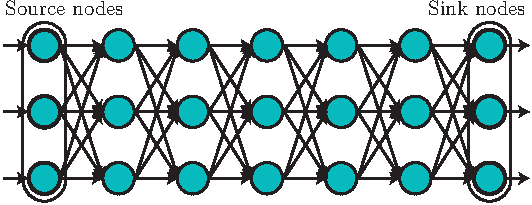
\includegraphics{figures/multiflow.pdf}
	\caption{A ``layered'' multi-commodity flow graph.}
	\label{fig:multiflow}
\end{figure}
It consists of 7 ``layers'' consisting of 3 nodes each, and there are 2 commodities. From each node at a given level, there is a directed edge to each node at the next level. Sources are composed of the nodes at the first level, while the nodes at the last level constitutes the sinks. The capacity for each commodity $c_i$ and edge $e$ is 0 with a probability of 5\% and otherwise drawn from a uniform distribution between 5 and 15, while the common capacity of the edge e is 0 with probability 25\% and otherwise a number drawn from the uniform distribution between $s$-10 and $s$, where $s$ is the sum of the individual capacities on that edge.

Similarly to Table~\ref{tab:projections}, Table~\ref{tab:multicom} shows the size of the original model (both as modelled and presolved) and the projections resulting from a flat and decomposed projection, respectively. Both projections finished and the time taken to make them is also shown. Figure~\ref{fig:multicom} shows the progression over time of the number of inequalities and number of variables left to be projected, for both the flat and decomposed projection algorithm.

\begin{table}[htbp]
\centering
\begin{tabular}{l|r@{ / }r@{ / }r@{ / }r|r}
\toprule
$\multirow{2}{*}{Model}$&\multicolumn{4}{c|}{Size}&{Time}\\
&ineqs (eqs)&vars&non-zeros&density&\\
\midrule
Original&204 (42)& 120& 444&2.17&-\\
Presolved& 59& 79& 201&3.41&-\\
Projected, decomposed& 17 (2)& 12& 61&3.59& 2h \phantom{9}9m \\
Projected, flat& 17 (2)& 12& 53&3.12& 17h 41m\\
\bottomrule
\end{tabular}
\caption{Size of projection of a multi-commodity flow model.}
\label{tab:multicom}
\end{table}

Also here, we see a reduction in the number of inequalities, variables and non-zero entries, of 3.5, 6.6, and 3.3/3.8 times, respectively (in both cases) compared to the presolved model. The density stays almost the same; for the decomposed model, the density increases with 5.3 \%, while the density decreases with 8.5\% for the flat projection.
This is not as big a reduction as for the VSMs, however, the unprojected models are also smaller to begin with. 

\begin{figure}
	\centering
		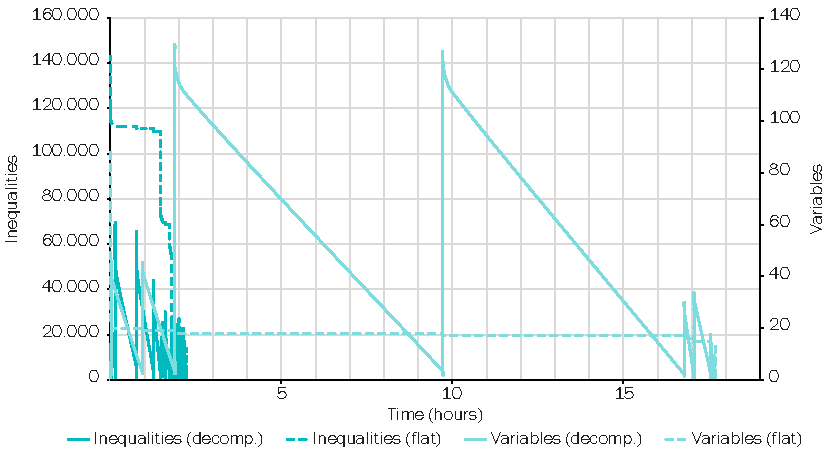
\includegraphics{figures/multicomGraph.pdf}
	\caption{The number of constraints and variables as a function of time during a flat and and a decomposed projection, respectievly, of a multi-commodity flow problem.}
	\label{fig:multicom}
\end{figure}

%\subsection*{Using projections}
%\red{Question: Under the assumption that the vessel is loaded with cargo in a valid configuration such that the utilization (or the revenue) is within 5 \% of the maximal value, what is the upper and lower bound (TEU) of each of the different types of containers?
%These values are obviously found by first finding the optimal value ( m = max \# TEU subject to stowage model constraints),
%and then -- for each type $\tau\in T$ -- maximizing, respectively minimizing, $y^\tau$ (whatever I called it) under the same constraints with the further constraint that \# TEU <= 0.95* m.  
%The table below shows the total time taken to find those upper and lower bounds for each type $\tau\in T$ after the maximal value has been found.} 

%\end{document}

%\subsection*{Projection of other block-structured systems/Multicommodity flow graphs} 
%\paragraph{For appendix}
%4 parts
%\begin{align*}
%\Bigg\{\bigg\{\Big\{\big\{\{1,2,3\},\{4,5\}\big\},\big\{\{6,7\}\big\}, LH\Big\},\Big\{\big\{\{8,9\}\big\},\big\{\{10,11\},\{12,13\}\big\}\Big\}\bigg\},\\
%\bigg\{\Big\{\big\{\{14,15\},\{16,17\}\big\},\big\{\{18,19\}\big\}\Big\},\Big\{\big\{\{20,21\},\{22,23\}\big\},\big\{\{24,25,26\}\big\}, RH\Big\}\bigg\}\Bigg\}
%\end{align*}

%6 parts:
%\begin{align*}
%\Bigg\{\bigg\{\Big\{\big\{\{1,2,3\},\{4,5\}\big\},\big\{\{6,7\},\{8,9\}\big\}, LH\Big\},\Big\{\big\{\{10,11\},\{12,13\}\big\}\Big\}\bigg\},
%\\
%\bigg\{\Big\{\big\{\{14,15\},\{16,17\}\big\},\big\{\{18,19\},\{20,21\}\big\}\Big\},\Big\{\big\{\{22,23\},\{24,25,26\}\big\}\Big\}\bigg\}\Bigg\}
%\end{align*}

%8 parts:
%\begin{align*}
%\Bigg\{\Bigg\{\bigg\{\Big\{\{1,2,3\}\Big\},\Big\{\{4,5\},\{6\}\Big\}\bigg\},\bigg\{\Big\{\{7\},\{8,9\}\Big\},\Big\{\{10,11\},\{12,13\}\Big\}\bigg\},LH\Bigg\},\\
%\Bigg\{\bigg\{\Big\{\{14,15\},\{16,17\}\Big\},\Big\{\{18,19\},\{20\}\Big\}\bigg\},\bigg\{\Big\{\{21\},\{22,23\}\Big\},\Big\{\{24,25,26\}\Big\}\bigg\},RH\Bigg\}\Bigg\}
%\end{align*}

%\end{document}
